\documentclass{beamer}
\usetheme{Madrid}

\usepackage{amsmath}
\usepackage{graphicx}
\usepackage{multicol}
\usepackage{multirow}

\usepackage{tikz}
\usetikzlibrary{shapes.geometric, arrows}
\usetikzlibrary{calc}

\usepackage{pgfplots}
\pgfplotsset{compat=1.18}

\pgfplotsset{
    report_style/.style={
    legend style={draw=none, font=\small},
    legend cell align=left,
    legend pos=north east,
    ylabel style={align=center, font=\bfseries\boldmath},
    xlabel style={align=center, font=\bfseries\boldmath},
    x tick label style={font=\bfseries\boldmath},
    y tick label style={font=\bfseries\boldmath},
    scaled ticks=false,
    every axis plot/.append style={thick},
    },
}

\usepackage[justification=centering]{caption}
\usepackage{subcaption}

\usepackage{xurl}

% default path to images and other assets
\graphicspath{{../assets/}}

% disable wrapping
\tolerance=1
\emergencystretch=\maxdimen
\hyphenpenalty=10000
\hbadness=10000

% number figure caption
\setbeamertemplate{caption}[numbered]

% display bib label in references
\setbeamertemplate{bibliography item}{\insertbiblabel}
\setbeamertemplate{bibliography entry title}{}
\setbeamertemplate{bibliography entry location}{}
\setbeamertemplate{bibliography entry note}{}

% Metadata
% ------------------------
\title[Connectomics segmentation]{Segmentation of 3D volume images for connectomics}
\subtitle{CMS Research project}

\author[Oleh Shkalikov]{Oleh Shkalikov\texorpdfstring{ (5102818)
\\[0.7em]{\small Supervisors: Jannik Irmai, David Stein}
\\{\small Chairholder: Prof. Dr. Bjoern Andres}}{}}

\institute[TU Dresden]{TU Dresden, MLCV chair}

\date{14 March, 2024}

\begin{document}

\frame{\titlepage}

% \begin{frame}
%     \frametitle{Agenda}
%     \tableofcontents
% \end{frame}

\section{Dataset description and analysis}
\begin{frame}
    \frametitle{The original dataset}
    \begin{minipage}{0.49\textwidth}
        The original image volumes are acquired by a focused ion beam scanning electron microscope (FIB-SEM)
        of the CA1 hippocampus region of the brain.
        The raw data has a shape \( 2048 \times 1536 \times 1065 \) and initially were used by
        \cite{lucchi2013learning,lucchi2011supervoxel} for mitochondria segmentation task.
    \end{minipage}
    \begin{minipage}{0.49\textwidth}
        \centering
        \begin{figure}
            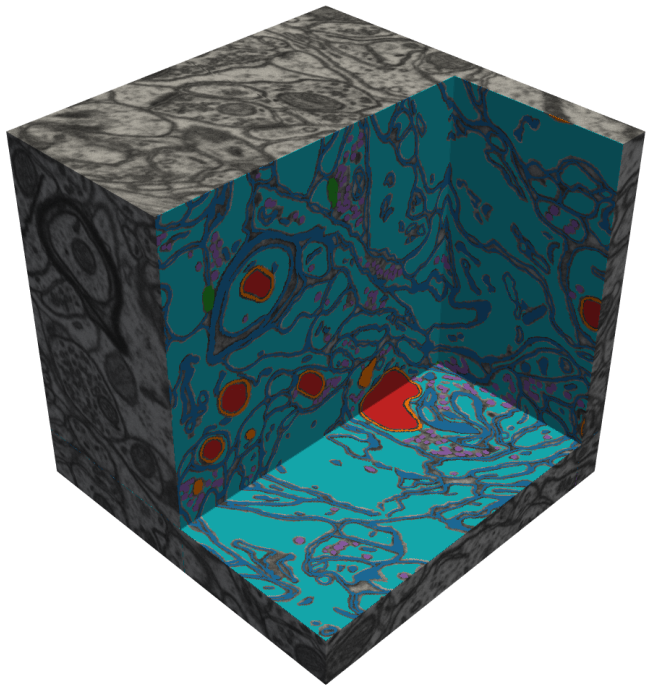
\includegraphics[width=0.8\textwidth]{cube_labeled.png}
            \caption{Connectomics volume image with provided labels\footnote{Credits to Jannik Irmai}}
        \end{figure}
    \end{minipage}
\end{frame}

\begin{frame}
    \frametitle{Labeling}
    \begin{minipage}{0.49\textwidth}
        The actual labeling has been performed on 9 slices of subvolumes into the following classes:
        \begin{enumerate}
            \itemsep0em
            \item cell cytoplasm
            \item cell membrane
            \item mitochondrion
            \item mitochondrion membrane
            \item synapse
            \item vesicle
            \item undefined (in the case where annotator was uncertain about the correct label)
        \end{enumerate}
    \end{minipage}
    \begin{minipage}{0.49\textwidth}

        \begin{figure}[ht]
            \centering
            \begin{tikzpicture}[scale=0.85]
                \begin{axis}[
                        report_style,
                        ybar,
                        xlabel={Class label},
                        ylabel={Number of pixels},
                        small
                    ]
                    \addplot+[] table[x=label,y=counts, col sep=comma] {../data/label_dist.csv};
                \end{axis}
            \end{tikzpicture}
            \caption{The distribution of labels for the train split}
            \label{fig:dist_labels}
        \end{figure}
    \end{minipage}
\end{frame}

\begin{frame}
    \frametitle{Example of a labeled slice}
    \begin{minipage}{0.49\textwidth}
        \centering
        \begin{figure}
            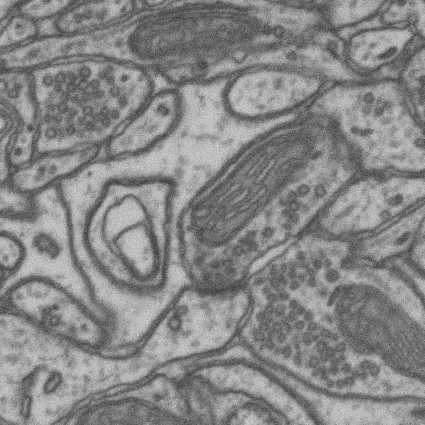
\includegraphics[width=0.9\textwidth]{original_slice.png}
            \caption{Original XY test slice}
        \end{figure}
    \end{minipage}
    \begin{minipage}{0.49\textwidth}
        \centering
        \begin{figure}
            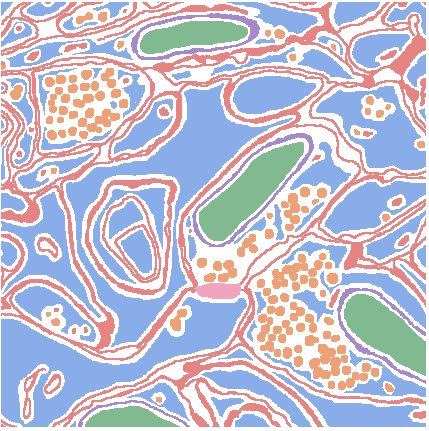
\includegraphics[width=0.9\textwidth]{labeled_slice.png}
            \caption{Labels for the test XY slice}
        \end{figure}
    \end{minipage}
\end{frame}

\begin{frame}
    \frametitle{Distributions of intensities}
    \begin{alertblock}{Are data normally distributed?}
        Statistical test of normality fails, so there is no evidence that data are normally distributed
    \end{alertblock}
    \begin{minipage}{0.49\textwidth}
        \centering
        \begin{figure}
            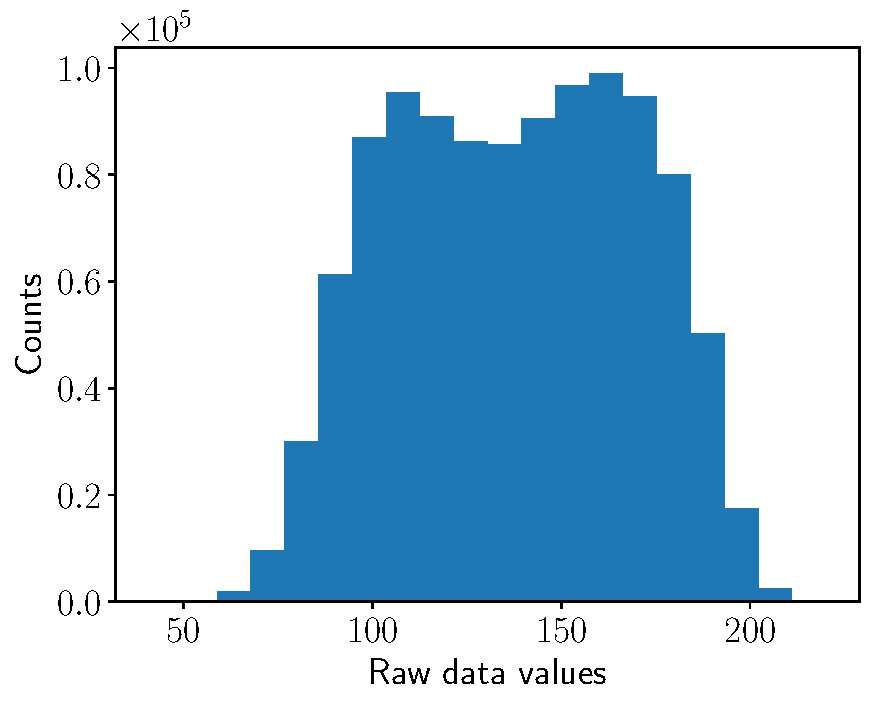
\includegraphics[width=0.9\textwidth]{raw_data_dist.pdf}
            \caption{Connectomics volume image with provided labels}
        \end{figure}
    \end{minipage}
    \begin{minipage}{0.49\textwidth}
        \centering
        \begin{figure}
            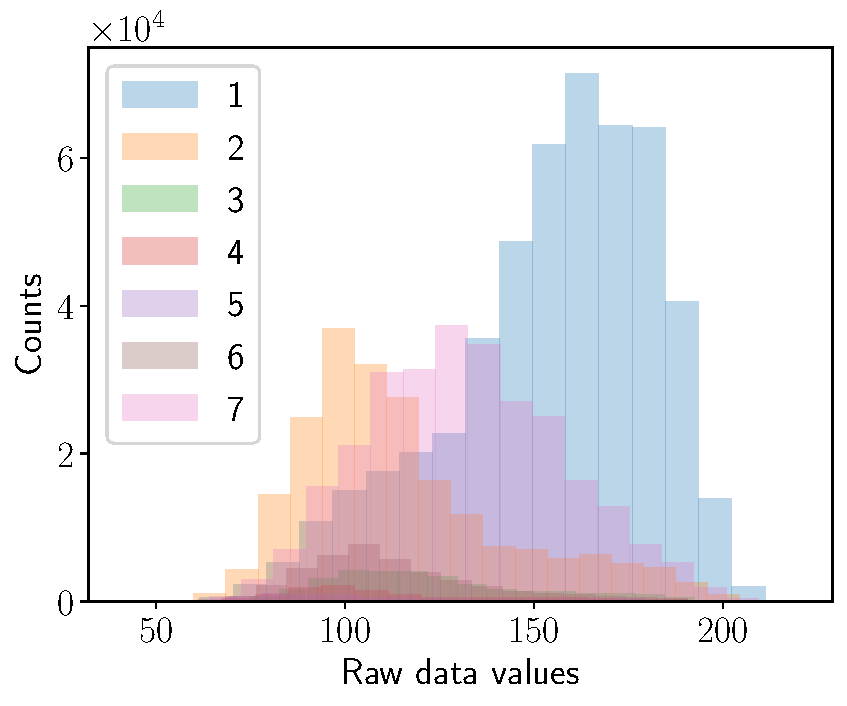
\includegraphics[width=0.9\textwidth]{raw_data_dist_per_label.pdf}
            \caption{Connectomics volume image with provided labels}
        \end{figure}
    \end{minipage}
\end{frame}

\begin{frame}
    \frametitle{Difference in intensities}
    \begin{block}{Means are different}
        Means of all class except cell membrane and mitochondrion membrane are
        different with high confidence levels.
    \end{block}
    \begin{table}[ht]
        \centering
        \begin{tabular}{|c|c|c|c|c|c|c|c| }
            \hline
            Label      & \textbf{1} & \textbf{2} & \textbf{3} & \textbf{4} & \textbf{5} & \textbf{6} & \textbf{7} \\
            \hline
            \textbf{1} & -          & 0          & 0          & 0          & 0          & 0          & 0          \\
            \hline
            \textbf{2} & 0          & -          & 0          & 0.175      & 0          & 0          & 0          \\
            \hline
            \textbf{3} & 0          & 0          & -          & 0          & 0          & 0          & 0          \\
            \hline
            \textbf{4} & 0          & 0.175      & 0          & -          & 0          & 0          & 0.0003     \\
            \hline
            \textbf{5} & 0          & 0          & 0          & 0          & -          & 0          & 0.0029     \\
            \hline
            \textbf{6} & 0          & 0          & 0          & 0          & 0          & -          & 0          \\
            \hline
            \textbf{7} & 0          & 0          & 0          & 0.0003     & 0.0029     & 0          & -          \\
            \hline
        \end{tabular}
        \caption{P-values of t-test for different labels combination}
        \label{tab:data_ttest}
    \end{table}
\end{frame}

\begin{frame}
    \frametitle{Limitations of the dataset}
    \begin{itemize}
        \item Labeling by non expert \textit{\( \Rightarrow \) there may be some mistakes in labeling}
        \item Limited size \textit{(even for artificial data generation via GANs)}
        \item Most interesting and hardest regions are unlabeled
        \item Labels only for slices \textit{\( \Rightarrow \) can not use SOTA segmentation models}
        \item One label per voxel \textit{\( \Rightarrow \) can not perform multi label classification}
        \item High class imbalance
    \end{itemize}
\end{frame}

\section{Methodology}

\begin{frame}
    \frametitle{}
    \begin{block}{The main idea}
        Instead of segmenting a whole input volume let's predict only the center voxel.
    \end{block}
\end{frame}

\section{Experiments}

\section{Directions of further research}

\section*{Conclusion}

\begin{frame}
    \frametitle{Conclusions}
\end{frame}

\section*{References}

\begin{frame}[allowframebreaks]
    \frametitle{References}

    \bibliographystyle{apalike}
    \bibliography{../references.bib}
\end{frame}


\end{document}